% !TEX root = knauss-vissuelizer.tex
\section{Introduction}

Large software projects often  need to collaborate across geographically distributed sites and depend on online communication to perform requirements related activities. 
More and more teams employ agile approaches that aim at discovering requirements iteratively and rely on frequent communication instead of requirements documentation. 
In such approaches, requirements are defined in the form of user stories, and ongoing discussions around these user stories serve as the main mechanism to clarify the meaning of requirements and to coordinate their implementation \cite{Cao2008}. 
Recording such discussions and decisions in online project repositories is an emerging best practice, not only in large and distributed projects \cite{Aranda2007}.
IBM\textsuperscript{\textregistered}'s Rational Team Concert\textsuperscript{\textregistered} project, with a large distributed team, is an example in which management mandates the recording of all critical communication in the project repository for future use \cite{Frost2007}. 
Consequently, online project repositories contain a valuable amount of requirements-related communication.

%Process-related issues, inadequate tool support or inadequate communication [refs) are common reasons for such problems. 
Communication to \emph{clarify} requirements is an important aspect of software projects, but a predominance of clarification communication late during the implementation of a requirement can indicate that the team does not have a sufficient understanding of the underlying requirement. When stakeholders continue to clarify the requirement because it is ambiguous, incomplete, or has frequent changes, the expected evolution of a requirement from an initial idea, through clarification, to design and full implementation, often stagnates. 
As a result, its implementation can be delayed, never completed or sometimes never get started. 
%Bikeshedding, also known as the Parkinson's law of triviality\cite{Parkinson1958} is another common situation in which developers give disproportionate weight and time to solving trivial issues and delay development. 
%An example from the RTC project (jazz.net) is the ongoing discussion of a large number of developers over the  text required in a UI element, and which blocked the development of this user story. 
%Late in the project a manager intervenes and makes a decision "we go with [...] for this iteration", after which development of the story is completed. 
%Although with a happy ending, many situations like this go unnoticed by managers. 
Current requirements management tools offer little support for identifying requirements with progression problems, thereby lowering the project manager's  ability to intervene in a timely manner.

%\begin{figure}[h]
%\begin{center}
%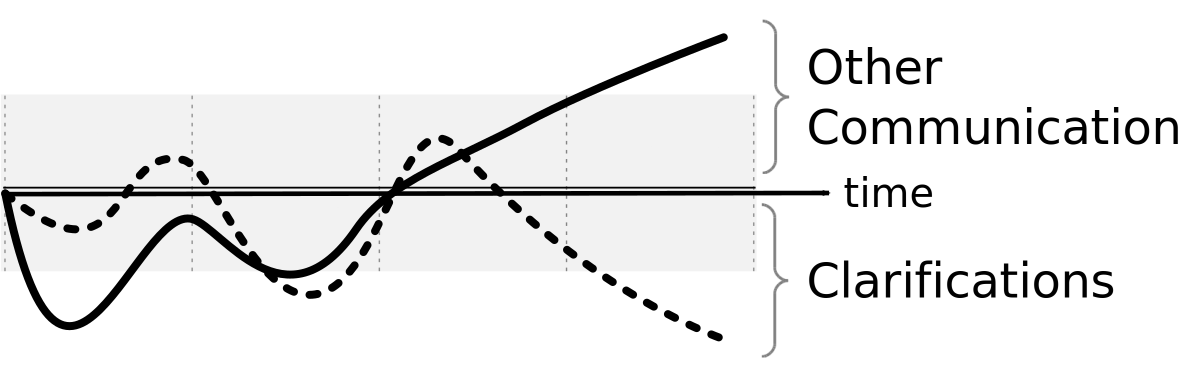
\includegraphics[width=0.7\columnwidth]{img/basic-pattern}
%\caption{Two different trajectories of reqts. communication}
%Predominance of clarifications in requirements-related communication may be problematic }
%\label{fig:basic-pattern}
%\end{center}
%\end{figure}

%Studying recorded online communication fills this gap by offering the potential to reveal patterns of communication that correlate to problematic situations around requirements development. 
In this demo we present a novel tool for analyzing online communication that helps managers to visualize the progression of clarification communication relative to other communication related to a particular requirement, thus providing support to differentiating between healthy and problematic requirements in the project. 
%Our \viss\ tool helps managers to analyze the content of stakeholder communication about  a particular requirement, identify specific instances of \emph{clarifying} communication, and examine the trajectory of clarifications (i.e. amount and progression) throughout the lifetime of a requirement. 
%Figure \ref{fig:basic-pattern} shows two distinct and quite different possible trajectories of \emph{clarifying} communication in the lifetime of a requirement. 
%While one would expect clarification to diminish as development of a requirement nears the end (solid line trajectory), its predominance throughout the requirement's life may be indicative of problematic requirements (dashed line trajectory). 
%The method proposed in this paper aims to identify these patterns automatically so that managers or involved stakeholders can be made aware of requirements that should be closely investigated.
\viss\ also visualizes stakeholder social networks related to a particular requirement to support the identification of communication breakdowns and experts for given topics.

%Figure \ref{fig:basic-pattern} depicts the characteristics of clarification communication related to a requirement (here: a story in Jazz).


%The contribution of this paper is the method for the detection and classification of clarification communication patterns, as well as a set of six communication patterns that we identified by applying our method in a large industrial project. 
%The remainder of the paper is structured as follows: Section \ref{sec:relatedwork} surveys related work in the study of communication in requirements engineering (RE), as well as related to information retrieval and automated classification techniques in RE. 
%Section \ref{sec:approach} introduces our research approach in studying requirements communication and the set of our techniques for the detection and classification of clarification  patterns. 
%We then describe the details of the industrial case study in which we applied our techniques in Sections \ref{sec:classification}, \ref{sec:visualization-and-patterns}, \ref{sec:recommendations} and \ref{sec:discussion}, and 
%give a detailed description of the three primary phases of our method: \emph{classification of requirements discussions}, \emph{clarification patterns development} and  \emph{pattern classification}.  
% conclude with future research steps in Section \ref{sec:conclusion}.

%\subsection{Background}
%The Jazz team uses Jazz as collaboration platform. It is the goal of the team to capture the entire communication in comments to \emph{workitems}. One of the workitem types, the \emph{story} contains requirements. Jazz follows an agile development approach, i.e. stories are refined during the project. This includes the decomposition in sub-workitems, most often of the workitem-type \emph{task}. 

%For a given requirement, the graph shows how the amount of clarification changes over time. 
%The example in the figure shows  a reoccurring characteristic that follows one of our six clarification communication patterns: the \emph{perfect clarification} pattern.


%Online communication to perform requirements related activities, such as elicitation, negotiation or development of requirements, is a critical part of large modern software projects. 
%Stakeholders in today's large software projects, most often at geographically distributed sites, largely rely on online communication in their collaboration. 
%Whether they follow an iterative discovery of requirements as in agile projects \cite{Cao2008}, or the time zone differences between stakeholders are too great to allow for frequent synchronous interaction (ref)2, or follow processes that mandate the recording of requirements communication online (ref3), these stakeholders perform various Requirements Engineering related activities through online communication. 

We conducted a preliminary evaluation in two ways. Firstly, we evaluated \viss's ability to correctly identify communication instances concerned with clarification and it's ability to derive meaningful visualizations of the clarification trajectory \cite{Knauss2012f}. 
Secondly, we showed  \viss's visualizations to software managers and asked them, whether the visualization was useful, if it did offer information they would have missed otherwise, and what actions they would perform based on the feedback, if any. 
This feedback lead to the development of additional features, e.g. social network analysis.

\begin{figure*}
\centering
\includegraphics[width=0.8\textwidth]{img/vissuelizer-screenshot}
\caption{The main window of the \viss\ shows a list of requirements (e.g. user stories in an issue tracker) and their clarification trajectories.}
\label{fig:screenshot}
\end{figure*}